\documentclass{article}
\usepackage{amssymb}
\usepackage{amsmath}
\usepackage{stix}
\usepackage{amsthm}
\usepackage{graphicx}
\usepackage[portuguese]{babel}
\usepackage{titling}

\usepackage{amsmath}
\usepackage{amsthm}
\usepackage{amssymb}
\usepackage{pgfplots}
\usepackage{amsfonts}
\usepackage[margin=2.5cm]{geometry}
\usepackage{graphicx}
\usepackage[export]{adjustbox}
\usepackage{fancyhdr}
\usepackage[portuguese]{babel}
\usepackage{hyperref}
\usepackage{lastpage}

\pagestyle{fancy}
\fancyhf{}

\hypersetup{
    colorlinks,
    citecolor=black,
    filecolor=black,
    linkcolor=black,
    urlcolor=black
}

\newtheorem*{sol*}{\underline{Solu\c c\~ao:}}
\newtheorem*{proof*}{\underline{Prova:}}
\renewcommand\qedsymbol{$\blacksquare$}

\rfoot{P\'agina \thepage \hspace{1pt} de \pageref{LastPage}}


\posttitle{\par\end{center}\vspace{30em}}

\begin{document}
\begin{figure}[ht]
	\minipage{0.76\textwidth}
		
\includegraphics[width=4cm]{../../icmc.png}
		\hspace{5cm}
		
\includegraphics[height=4.9cm,width=4cm]{../../brasao_usp_cor.jpg}
	\endminipage	
\end{figure}

    \begin{center}
        \vspace{1cm}
        \LARGE
        UNIVERSIDADE DE S\~AO PAULO

        \vspace{1.3cm}
        \LARGE
        INSTITUTO DE CI\^ENCIAS MATEM\'ATICAS E COMPUTACIONAIS - ICMC

        \vspace{1.7cm}
        \Large
        \textbf{O Problema da Sala Reprovada}\\ 
        \large Uma Releitura do Problema dos 100 Prisioneiros

        \vspace{1.3cm}
        \large
        \textbf{Renan Wenzel - 11169472}

        \vspace{1.3cm}
        \large
        \textbf{Pedro Rios - prios@icmc.usp.br}

        \vspace{1.3cm}
        \today
    \end{center}
    \newpage  
    
    \tableofcontents
    
    \newpage
    \section{Introdu\c c\~ao ao Problema}
    \subsection{Enunciando a Problem\'atica}
        \paragraph{}Imagine que uma turma de Fundamentos de Matem\'atica de 30 alunos est\'a com m\'edia 0. Todos da sala encontram-se desolados, achando que ser\~ao
        reprovados sem chance alguma de sucesso. Vendo esta situa\c c\~ao, o professor, em toda sua complac\^encia, resolvo propor a seguinte salva\c c\~ao aos desesperados 
        alunos:
        \begin{quote}
            ``\textit{Organizei nas 30 carteiras dessa sala n\'umeros. Embaixo delas, h\'a um bilhete com um n\'umero aleat\'orio que n\~ao se repete. Para cada n\'umero, 
            h\'a um aluno, e cada um de voc\^es possui exatamente 15 chances de encontrar o n\'umero correspondente. Se todos encontrarem os n\'umeros respectivos dentro 
            dessas tentativas, aumentarei a nota de todos para 10, mas, caso contr\'ario, a nota permanecer\'a 0 sem oportunidade de uma prova substitutiva.}"
        \end{quote}
        \paragraph{}Os alunos aceitaram o desafio e come\c caram a trabalhar no problema. Fica a pergunta para o leitor: Qual \'e a melhor estrat\'egia que eles podem usar?
    \subsection{Abordagem Inicial}
        \paragraph{}A primeira ideia que eles tiveram foi a de todos checarem carteira por carteira aleatoriamente; Afinal, essa \'e a primeira ideia que viria \`a mente 
        de praticamente qualquer um. S\~ao 15 chances para 30 carteiras, ou seja, cada aluno tem $1 \fracslash 2 = 50\%$ de chance de encontrar seu n\'umero, totalizando  
        $$
            \frac{15}{30} = \biggl(\frac{1}{2}\biggr)^{30} \approx 
        $$
        $$
            \approx 0,000,000,000,9 = 9.10^{-10}.
        $$
        Pra compara\c c\~ao, as chances de ganhar na Mega-Sena s\~ao de aproximadamente $0,000,000,02 = 2^{-8}$, uma ordem 100 vezes maior que as chances dos alunos ganharem.
        Em conclus\~ao, eles precisam encontrar outra estrat\'egia, e a combinat\'oria entra para calcularmos as chances deles ganharem com uma estrat\'egia melhor.

    \section{Uma Solu\c c\~ao Aceit\'avel ao Problema}
    \subsection{O Algor\'itmo para Resolver}
        \paragraph{}O princ\'ipio por tr\'as da solu\c c\~ao \'otima \'e criar um la\c co com os n\'umeros das carteiras tal que em algum momento antes do fim, 
        o n\'umero do aluno ir\'a aparecer para ele. Isso pode ser escrito num algoritmo da seguinte forma: \\
        \textbf{O estudante abre a carteira com o seu pr\'oprio n\'umero;}\\
        \textbf{Se o n\'umero for o dele, parar;}\\
        \textbf{Se n\~ao, o estudante segue at\'e a carteira que tem o n\'umero que ele encontrou.}\\
        Com os ciclos organizados desta maneira, \'e garantido que o aluno esteja num c\'iclo que contenha seu n\'umero, afinal o ciclo s\'o termina quando o mesmo for
        encontrado. A quest\~ao restante \'e se esse n\'umero pode ser encontrado em menos de 15 tentativas, ou seja, o maior ciclo feito desta forma tem que ter 
        tamanho de no m\'aximo 15 para que os alunos consigam o 10. 
    \subsection{Um Exemplo do Aluno Enumerado 13}
    \paragraph*{Exemplo de Sucesso}Considere um aluno espec\'ifico que deve encontrar o n\'umero 13. Ele anda at\'e a carteira 13 e encontra o n\'umero 10 escrito, fazendo com que ele ande 
    at\'e a carteira 10. Olhando embaixo dela, ele acha o n\'umero 5, ou seja, ele deve andar at\'e a quinta carteira e conferir o n\'umero abaixo dela, marcado
    29. Ao chegar na vig\'esima nona mesa, ele finalmente encontra o seu n\'umero, 13. Uhul, o aluno 13 conseguiu passar!
    \begin{figure}[h]
        \centering
        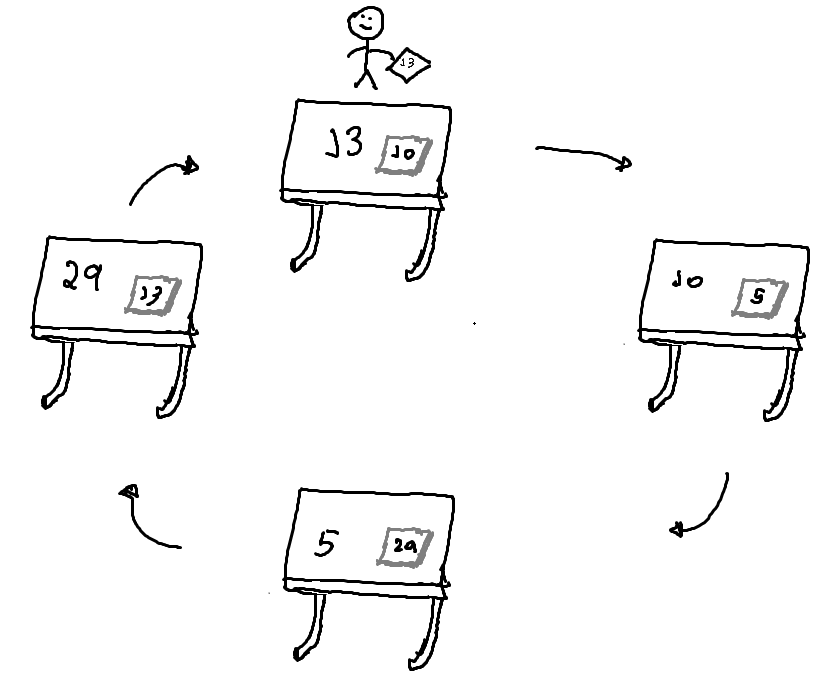
\includegraphics[width=5cm, height=5cm]{Win.png}
        \caption{N\'umero 13 Ganha}
    \end{figure}
    
    \paragraph*{Exemplo de Falha}Dessa vez, considere o mesmo aluno com n\'umero 13. Ele anda at\'e a carteira 13 e encontra o n\'umero 10 escrito, fazendo com que ele
    ande at\'e a carteira 10. Olhando embaixo dela, ele acha o n\'umero 5, ou seja, ele deve andar at\'e a quinta carteira e conferir o n\'umero abaixo dela, marcado
    29. Ao chegar na vig\'esima nona mesa, ele acha o n\'umero 5, e fica repetindo isso at\'e esgotar as 15 tentativas. Para fins de trag\'edia, na d\'ecima sexta tentativa,
    em que ele est\'a na mesa de n\'umero 9, ele finalmente encontra seu n\'umero. Por\'em, como tomou 16 chances at\'e ele achar, o n\'umero 13 n\~ao ganhou, e todos da
    sala permaneceram com 0. $:(.$
    \begin{figure}
        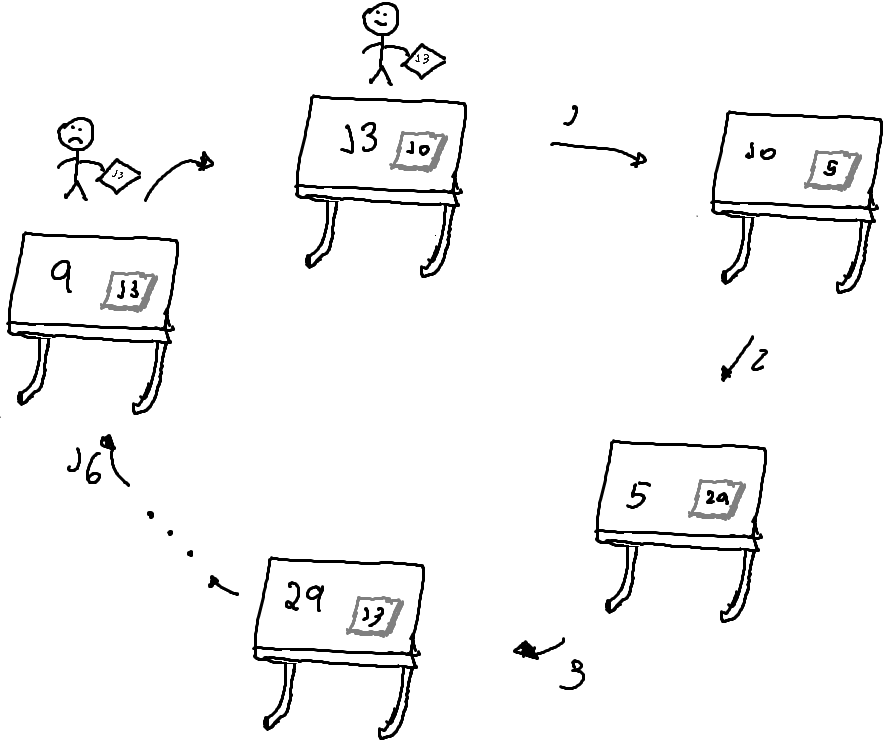
\includegraphics[width=5cm, height=5cm]{Lose.png}
        \centering
        \caption{N\'umero 13 Perde}
    \end{figure}

    \newpage
    \subsection{Calculando as Chances de Sucesso}    

        \paragraph{}Considere uma permuta\c c\~ao de 1 a 30. Se um dos ciclos tiver tamanho maior que 15, ent\~ao os outros todos devem ter tamanhos menores do que 15 para manter
        consist\^encia nessa permuta\c c\~ao. 
        
        \paragraph{}Em outras palavras, seja d o tamanho deste c\'iclo, ou seja, $d > 15$. O conceito de escolha nos permite calcular quantas 
        formas um aluno pode cair neste c\'iclo, que ser\'a dada por $\binom{30}{d}$ e, sendo todas as poss\'iveis permuta\c c\~oes do ciclo \'unicas, ou seja, removendo
        as permuta\c c\~oes sim\'etricas, existem $(d-1)!$ formas de organizar os n\'umeros do ciclo de falha no jogo. Ademais, para os outros ciclos, seus n\'umeros estar\~ao
        organizados de $(30 - (d - 1) - 1) = (30 - d)!$ formas diferentes, j\'a que estamos excluindo as permuta\c c\~oes anteriores.

        \paragraph{}Logo, para um ciclo de tamanho $l > 15$, existem 
        $$
        (d-1)!(30-d)!\binom{30}{d} = \frac{30!(30-d)!(d-1)!}{d!(30-d)!} = \frac{30!(30-d)!(d-1)!}{d(d-1)!(30-d)!} = \frac{30!}{d}
        $$
        formas de escrever seus n\'umeros. 

        \paragraph{}Com esta informa\c c\~ao, vamos encontrar a chance de fracasso no jogo, ou seja, iremos somar todas as chances de falha e dividir cada uma pelo n\'umero total
        de permuta\c c\~oes, isto \'e, 
        $$
            \frac{30!}{30!16} + \frac{30!}{30!16} + \cdots + \frac{30!}{30!29} + \frac{30!}{30!30} = \frac{1}{16} + \cdots + \frac{1}{30} \approx 0,677.
        $$
        Por fim, como todo bom estudante de probabilidade, se sabemos a chance de fracasso, basta subtrair ela de um para encontrar as chances de sucesso, que acabam sendo
        $$
            P(\text{sucesso}) = 1 - 0,677 = 0,323 \approx 32\%.
        $$
    \subsection{Considera\c c\~oes finais}
        \paragraph{}Os alunos, ap\'os compreenderem essa estrat\'egia, decidem implement\'a-la, efetivamente aumentando as chances de sucesso de $9.10^{-10}$ para $3,2.10^{-1}$, o que
        resulta em um aumento de 
        $$
            \frac{3,2.10^{-1}}{9.10^{-10}} \approx 0,35.10^{9} = 3,5.10^{8}
        $$
        vezes (consideravelmente maior!). 

    \begin{center}
        \textbf{\MakeUppercase{Esse trabalho foi baseado no ``Problema dos 100 Prisioneiros". Se quiser saber mais, seguem abaixo algumas fontes.}}
    \end{center}

    \begin{thebibliography}{Xyz12}
        \item MULLER, D. \textbf{The Riddle That Seems Impossible Even If You Know The Answer}. Youtube, 30 de Junho de 2022. Dispon\'ivel em: https://www.youtube.com/watch?v=iSNsgj1OCLA. Acesso em: 18 de Julho de 2022.
        \item STANLEY, R.P. \textit{Algebraic Combinatorics: Walks, Trees, Tableaux, and More}. Springer. Acesso em: 18 de Julho de 2022.
    \end{thebibliography}
\end{document}